\documentclass[11pt,letterpaper]{article}
\usepackage[lmargin=1in,rmargin=1in,tmargin=1in,bmargin=1in]{geometry}
\usepackage{../style/homework}
\usepackage{../style/commands}
\setbool{quotetype}{false} % True: Side; False: Under
\setbool{hideans}{true} % Student: True; Instructor: False

% -------------------
% Content
% -------------------
\begin{document}

\homework{17: Due 11/23}{I was on the street. This guy waved to me, and he came up to me and said, `I'm sorry. I thought you were someone else.' And I said, `I am.'}{Demetri Martin}

% Problem 1
\problem{10} Sketch the function $y= \log_2 x$. 
	\[
	\fbox{
	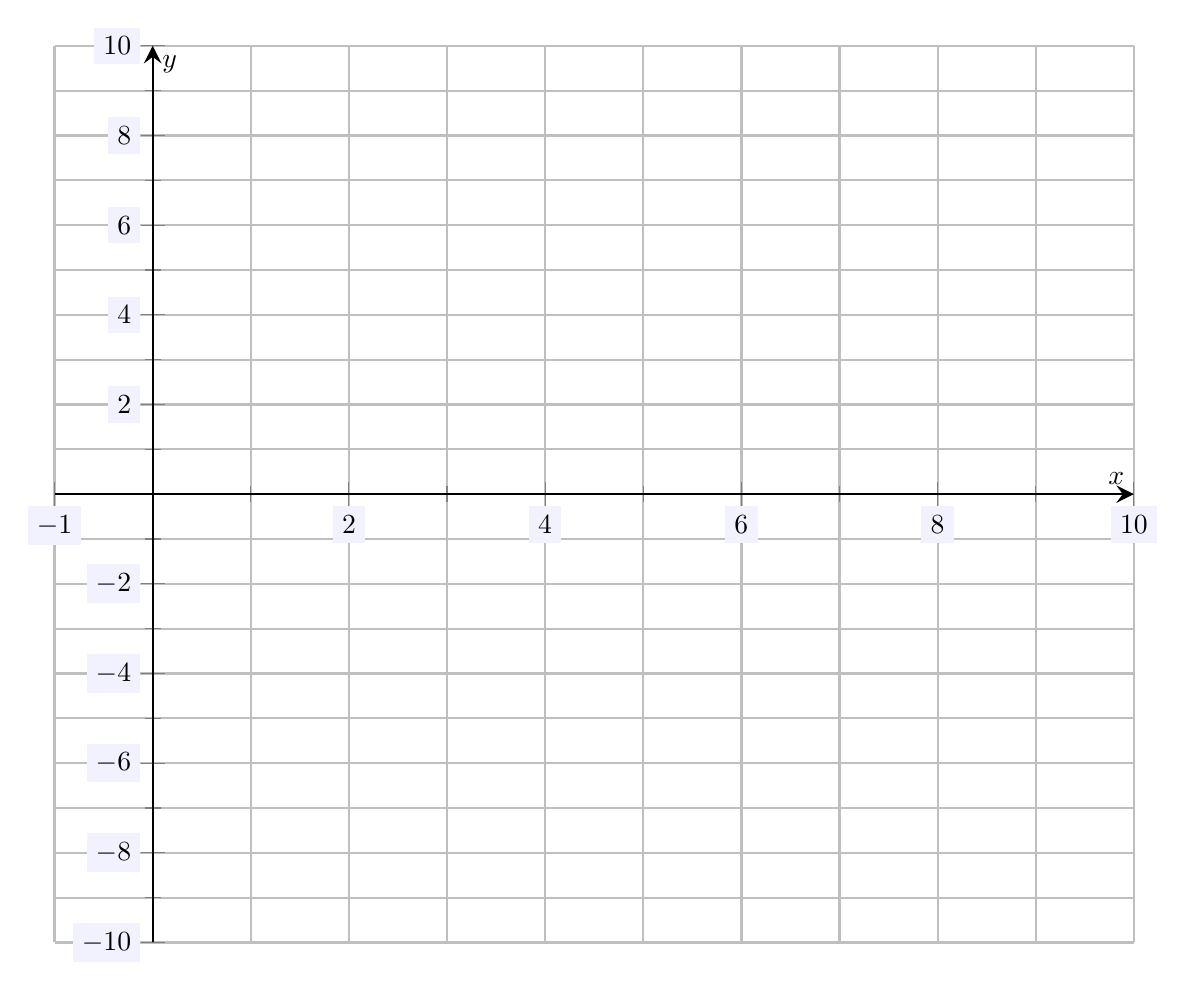
\begin{tikzpicture}[scale=2,every node/.style={scale=0.5}]
	\begin{axis}[
	grid=both,
	axis lines=middle,
	ticklabel style={fill=blue!5!white},
	xmin= -1, xmax=10,
	ymin= -10, ymax=10,
	xtick={-1,0,2,4,6,8,10},
	ytick={-10,-8,...,10},
	minor tick = {-10,-9,...,10},
	xlabel=\(x\),ylabel=\(y\),
	]
	\end{axis}
	\end{tikzpicture}
	}
	\] \pspace





\newpage





% Problem 2
\problem{10} Compute the following:
\begin{enumerate}[(a)]
\item $\log_4 4 - \log_6 1$
\item $\log_5 25$
\item $\log_3 \dfrac{1}{81}$
\item $\log_9 \sqrt{3}$
\item $\ln e^{2/3}$
\end{enumerate} \pspace





\newpage 





% Problem 3
\problem{10} Expand the following logarithm completely by expressing it as a sum or difference of logs. Your answer should not include any exponents.
	\[
	\log_3 \left(\dfrac{\sqrt[6]{x}}{3y^4}\right)
	\] \pspace





\newpage





% Problem 4
\problem{10} Rewrite the expression below as a single logarithm. 
	\[
	\frac{1}{2} \ln x - \ln 1 + 3\ln(x+2) - \ln(1 - x)
	\] \pspace


%\printpoints
\end{document}